\section{Data Modelling}
Coming up with a domain model is a process that can provide clarity and direction for a software system, even on a small scale such as in a library. 

\subsection{Data Model Overview}
In order to capture the data model in an object-oriented programming language, a UML diagram was maintained as the implementation went along in order to keep track of relationships between the classes. 
% As a general rule of thumb, all the fields were made public including those required by the constructors, and the methods of the classes were all \textit{getters}, i.e. \\

\subsubsection*{Location}
A \textit{Location} is defined by a geographical \textit{latitude} and \textit{longitude} and represents a real-life location.

\subsubsection*{Cluster}
A \textit{Cluster} is created from a collection of \textit{Locations}. This class serves as an auxiliary class for clustering based on median \textit{latitude} and \textit{longitude}.

\subsubsection*{Single Location Point (SLP)}
A \textit{Single Location Data Point} (SLP) is a time-stamped \textit{Location}. By having a time-stamp, a collection of SLPs may be ordered and grouped by the time of day. In essence, the SLP is a Data Transfer Object (DTO) \footnote{\url{https://martinfowler.com/eaaCatalog/dataTransferObject.html}} which is used to transfer GPS data from an arbitrary Location plugin to the \textit{Mobility Features Package}.

\subsubsection*{Hour Matrix}
An \textit{Hour Matrix} is a matrix with 24 rows and columns equal to the number of places of some period. The \textit{Hour Matrix} class is used to calculate the \textit{Routine Index} feature, as well as to identify the \textit{Home Cluster}, which is the place most visited during 00:00 and 06:00. An Hour Matrix is constructed from a list of \textit{Stops} which all have the same date.

\subsubsection*{Stop}
% A \textit{Stop} is a visit at a known \texit{Place} (see below) for an extended period of time. A \textit{Stop} is defined by a location that represents the centroid of a collection of data points, from which a \textit{Stop} is created. In addition a \textit{Stop} also has an \textit{arrival}- and a \textit{departure} time-stamp, representing when the user arrived at the place and when the user left the place. From the arrival- and departure timestamps of the \textit{Stop} the duration can be computed.

\subsubsection*{Place}
% A \textit{Place} defined as a group of stops that were clustered by the DBSCAN algorithm \cite{density-based-1996}. From the cluster of stops, the centroid of the stops can be found, i.e. the center location. In addition, it can be computed how long a user has visited a given place by summing over the duration of all the stops at that place.

\subsubsection*{Move}
% A \textit{Move} is the displacement of the user from stopping $s_a$ to stop $s_b$ in which the user passes through a series of SLPs. Given the distance traveled from stop $s_a$ to stop $s_b$, in addition to the departure of $s_a$ and the arrival at $s_a$ the average speed at which the user traveled can be derived. 

\subsubsection*{Mobility Context}
A \textit{Mobility Context} is a collection of features which are derived from a set of intermediate features, where the \textit{Stops} and \textit{Moves} are from a specific date. The \textit{Places} is derived from multiple dates for reasons which will be explained in the implementation details. In addition, a set of \textit{Mobility Contexts} from previous dates can be provided as an optional parameter. A Mobility Context contains the mobility features, although the \textit{Routine Index} is only available if an array of the set of \textit{Mobility Contexts} was provided as a parameter, which is due to the feature depending on the data from previous days in order to compare them.

\subsection{UML Diagram and Discussion}

\begin{figure}[h]
    \centering
    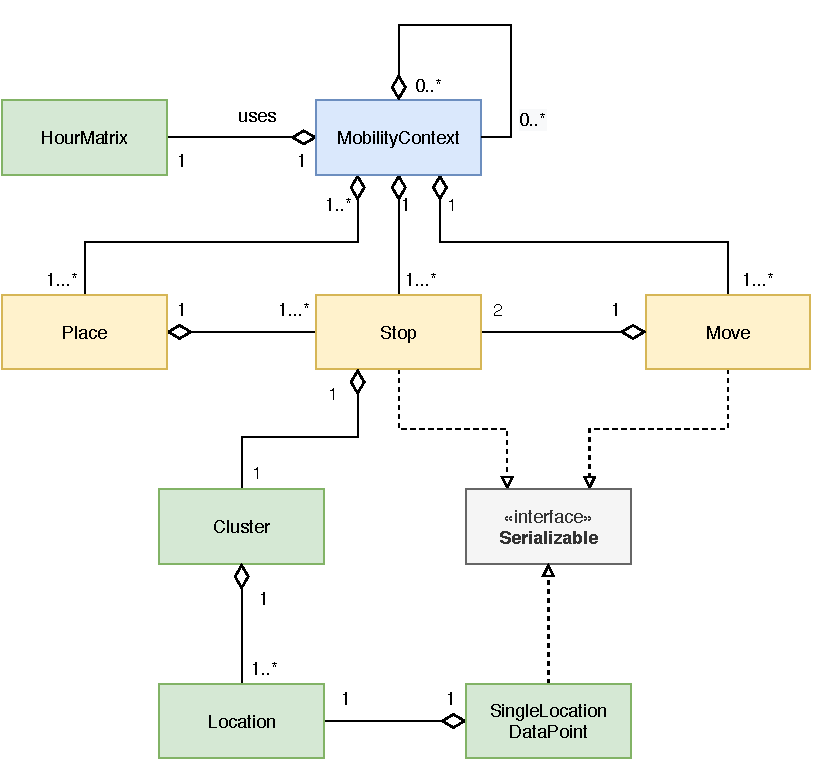
\includegraphics[width=0.7\textwidth]{./images/uml-mobility.pdf}
    \caption{UML diagram for the classes used in the \textit{Mobility Features Package}}
    \label{fig:my_label}
\end{figure}

The data model could be modified such that a Place contained a list of \textit{Stops} made at that place, rather than using both \textit{Places} and \textit{Stops} for instantiation of \textit{Mobility Context}. This would mean grouping the \textit{Stops} by Place rather than date, and would require filtering to take place every time a \textit{Mobility Context} object is created, to remove all Stops, not on that specific date. In a real-world scenario the application developer will likely have the SLPs for the current day available, and from those the \textit{Stops} today can be generated which means no filtering is required. Grouping \textit{Stops} into places would however lead to a nicer data model, but a design choice was made in favor of less computation. 


